\section{LED Driver}
The brick sorter relies on the varying reflective properties of different colours. Using a variety of different colour LEDs will enable the sorter to detect different colour bricks. This section will describe in detail the decisions made in designing the circuit used for the LEDs and the photo diode as well as presenting the code responsible for driving the LEDs. 

\subsection{Circuit Design}
\begin{figure}[h!]
	\begin{center}
		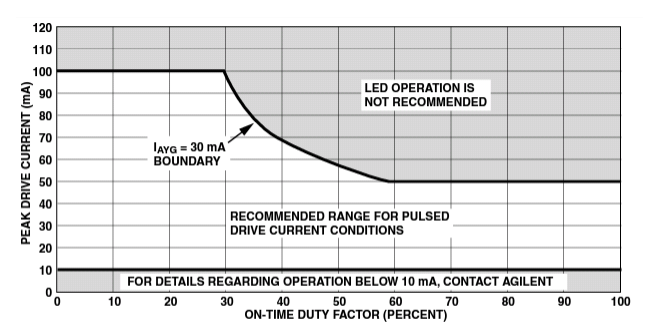
\includegraphics[width=\linewidth]{images/overdrive}
	\end{center}
	\caption{The white region denotes the area in which the LED can safely be driven.}
	\label{fig:overdrive}
\end{figure}
The switching of the LEDs is done using bipolar junction transistors (BJTs). The BJTs are wired as a simple switching circuit as in figure \ref{circ:ledswitch}. $V_{\text{c}}$, the switching signal, will be generated using an FPGA.
In order to achieve the highest possible light intensity from the LEDs they will be overdriven. Figure \ref{fig:overdrive} is an excerpt from \cite{avago}. This graph shows that the LEDs can be safely driven at 100mA so long as the duty cycle of $V_{\text{c}}$ does not exceed 30\%. Driving the LEDs at 100mA implies that $I_c=100\text{mA}$. 

For a BJT:
\begin{eqnarray}
I_c=&I_b\cdot h_{\text{FE}}\\
I_b=&\frac{V_{\text{c}}-V_{be}}{R_1}
\end{eqnarray}
Looking at the datasheet of the BC547b the dc current gain of this transistor is found to be
\begin{eqnarray}
	h_{\text{FE}}=200 \Rightarrow I_b = 0.5\text{mA}
\end{eqnarray}
Lastly, according to figure \ref{fig:vbe} from the datasheet of the BC547b, when $I_c = 100$mA $V_{be}=0.8$v.
Since the BJT is used as a switch it is desirable that it is driven to saturation quickly to avoid dissipating power in the component. Therefore, $I_b$ is doubled and 
\begin{eqnarray}
	R_1 = \frac{V_{\text{c}}-V_{be}}{I_b\cdot 2} = 2.5\text{k}\Omega
\end{eqnarray}

\begin{figure}[h!]
	\centering
	\begin{subfigure}[b]{.48\linewidth}
		\begin{circuitikz}
			\draw (0,0) 
			node[npn](npn1){}
			(npn1.base) ++(-2,0) node[name=r1left]{}
			to[R=$R_1$,o-,i=$I_b$] ++(2,0) ++(-2,0)node[left]{$V_{\text{c}}$}
			(npn1.base) ++(0.75,0) node[right]{BC547b}
			(npn1.emitter) 
			node[ground](GND){}
			(npn1.collector) ++(0,4) node[name=d_top]{}
			to[D=$LED$,o-]++(0,-2) 
			to[R=$R_2$,i=$I_c$]++(0,-2)
			(d_top) node[above]{$V_{cc}$}
			;\end{circuitikz}
		\caption{Switching circuit for single LED}
		\label{circ:ledswitch}
	\end{subfigure}
	\begin{subfigure}[b]{.48\linewidth}
		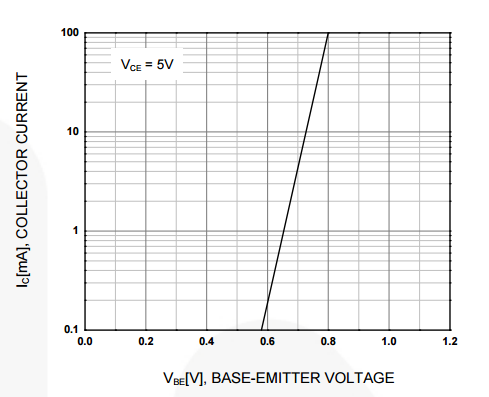
\includegraphics[width=\linewidth]{images/vbe}
		\caption{Graph of $I_c$ as a function of $V_be$.}
		\label{fig:vbe}
	\end{subfigure}
	\caption{(a)LED Circuit, three of these are combined to drive the red, green and blue LEDs used in this application. (b) Graph from the datasheet of the BC547p showing the correlation between collector current and base-emitter voltage.}
\end{figure}
\begin{figure}[h!]
	\begin{center}
		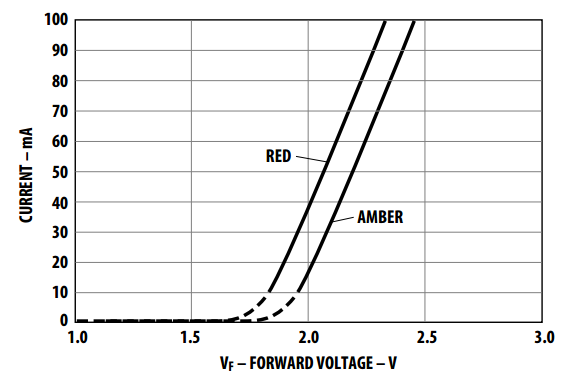
\includegraphics[width=0.75\linewidth]{images/redvd}
	\end{center}
	\caption{Current as a function of forward voltage for the red diode.}
	\label{fig:ledcurrent}
\end{figure}
Finding $R_2$ is done using the datasheets of the LEDs. figure \ref{fig:ledcurrent} shows the correlation between the voltage drop across the diode and the current through the diode.
According to these figures the red LED will have a voltage drop $V_d = 2.3$v and the green and blue LEDs will $V_d = 4$v. This results in 
\begin{eqnarray}
	R_{2\_\text{red}}=& \frac{V_{cc}-V_d}{I_c} &= 97\Omega \\
	R_{2\_\text{green}}=&R_{2\_\text{blue}} = \frac{V_{cc}-V_d}{I_c} &= 80\Omega
\end{eqnarray}

This next part of the circuit is responsible for detecting the reflected light and amplify the signal generated by the photodiode such that it can be processed by the ADC. A diagram of the circuit used can be seen in figure \ref{circ:unfiltered}.
The output voltage of this circuit is determined by:
\begin{eqnarray}
	V_{\text{out}}=&I_{\text{in}}\cdot R_f\\
	R_f =& R_1+R_{\text{pot}}
\end{eqnarray}
When an LED is flashed onto a same-coloured brick, the output of the op-amp is expected to be $V_{\text{out}} = V_{\text{sat}}$, the saturation voltage. By experimentation this was found to be $V_{\text{sat}}=3.78$v.

$I_{\text{in}}$ was determined by making the circuit as seen in figure \ref{circ:iinmeasure}. By reflecting the light from the LEDs off of the bricks and onto the photodiode, a current is induced in the circuit and a voltage drop can be measured across the 1k$\Omega$ resistor the maximum current to be expected generated from the photodiode was found to be $I_{\text{in}}=10\mu$A.
\begin{figure}[h!]
	\centering
	\begin{circuitikz}
		\draw(0,0) 
			to[short] ++(2,0)
				to[R=1k$\Omega$] ++(0,-2)
					to[short] ++(-2,0) 
						to[pD] ++(0,2) coordinate(d_right)
			(d_right) ++(-1.5,0) to[short,-o] ++(-1,0)
			(d_right) ++(-1.5,0) to[lamp] ++(0,-2)
				to[short,-o] ++(-1,0)
	;\end{circuitikz}
	\caption{Circuit used for measuring the max current expected to be generated from the photo diode when in operation.}
	\label{circ:iinmeasure}
\end{figure}

This results in $R_f=378\text{k}\Omega$, however, it was found that applying this resistor causes the blue brick to also saturate the op amp when shining the green LED. Additionally, when mounting the LED assembly to the acrylic slide, the slide itself was found to enlarge $I_{\text{in}}$ by a significant margin. Due to these factors $R_f$ was finally dimensioned using a 1M$\Omega$ potentiometer. \todo{And final value is?!}

\begin{figure}[h!]
  	\centering
	\begin{subfigure}[b]{.49\linewidth}
		\resizebox{\linewidth}{!}{
			\begin{circuitikz}
				\draw(0,0) 
					node[op amp] (opamp) {}
				(opamp.-) ++(-2,-1) 
					node[ground]{} to[short] ++(0,1)
						to[pD] (opamp.-)
				(opamp.-) to[short] ++(0,1) coordinate(capleft)
					to[R=$R_1$] ++(2,0)
						to[vR=$R_\text{pot}$] ++(2,0) coordinate(pot)
				(opamp.out) -| (pot) coordinate(conn)
					to[short] (pot)
				(opamp.+) to[short] ++(0,-0.5)
					node[ground]{}
			;\end{circuitikz}
		}
		\caption{Unfiltered version.}
		\label{circ:unfiltered}		
	\end{subfigure}
	\begin{subfigure}[b]{.49\linewidth}
		\resizebox{\linewidth}{!}{
			\begin{circuitikz}
				\draw(0,0) 
				node[op amp] (opamp) {}
				(opamp.-) ++(-2,-1) 
				node[ground]{} to[short] ++(0,1)
				to[pD] (opamp.-)
				(opamp.-) to[short] ++(0,1) coordinate(capleft)
				to[R=$R_1$] ++(2,0)
				to[vR=$R_\text{pot}$] ++(2,0) coordinate(pot)
				(opamp.out) to[short] (opamp.out -| pot) coordinate(conn)
				to[short] (pot)
				(opamp.+) to[short] ++(0,-0.5)
				node[ground]{}
				(capleft) to[short] ++(0,1) coordinate(capleftup)
				to[C=$C_f$] (capleftup -| pot)
				to[short] (pot)
				;\end{circuitikz}
		}
		\caption{Filtered version.}
		\label{circ:filtered}
	\end{subfigure}
   	\caption{Photo diode amplifier circuit}
   	\label{circ:photodiode}
\end{figure}

Table \ref{tab:ledtable} shows the various responses of the photodiode when exposed to the different LEDs and bricks.

\begin{table}
	\centering
	\begin{tabular}{| c | c | c | c | c |}
		\hline
		\diagbox{LED}{BRICK}& R & G & B & A\\
		\hline
		R & 2.97 & 1.11 & 1.30 & 1.66\\
		\hline
		G & 1.71 & 3.34 & 2.81 & 2.49\\
		\hline
		B & 1.78 & 2.00 & 3.86 & 2.38\\
		\hline
	\end{tabular}
	\caption[Response from photodiode circuit.]{Response from photodiode circuit. Each colour LED; red, green and blue is flashed while each colour brick is used as the reflective surface.}
	\label{tab:ledtable}
\end{table}
\subsection{Circuit Testing}
In testing, a significant amount of oscillation appeared on the output of the op amp. See figure \ref{fig:oscillation}. To avoid issues when digitizing the signal with the ADC, it will be filtered by applying a compensation capacitor in parallel with $R_f$, see figure \ref{circ:filtered}.

\begin{figure}[h!]
	\centering
	\begin{subfigure}{\linewidth}
		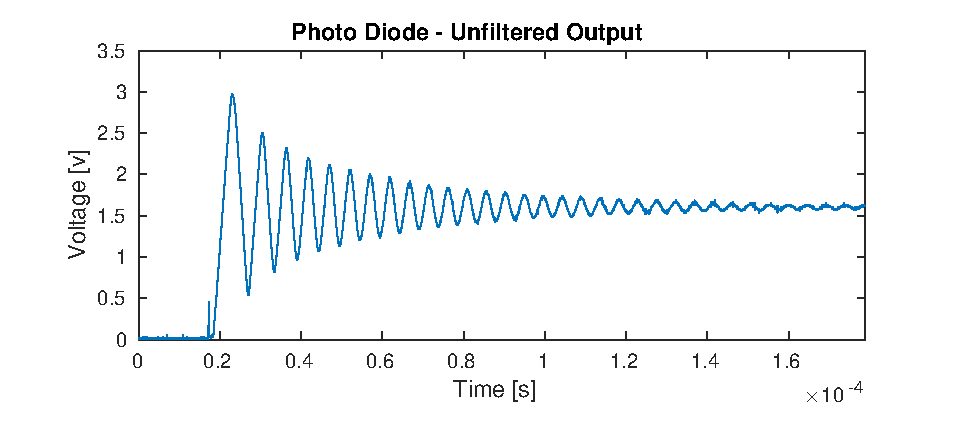
\includegraphics[width=\linewidth]{images/unfiltered}
		\caption{Unfiltered output.}
		\label{fig:oscillation}
	\end{subfigure}\\
	\begin{subfigure}{\linewidth}
		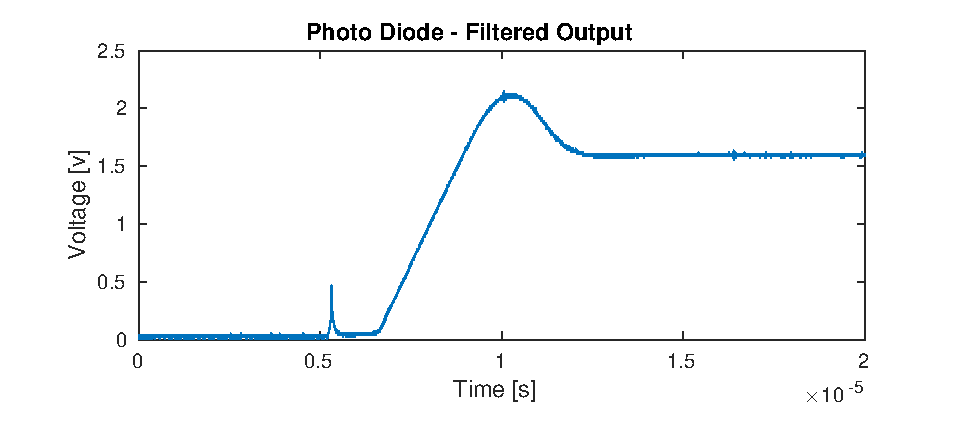
\includegraphics[width=\linewidth]{images/filtered}
		\caption{Filtered output.}
		\label{fig:nooscillation}
	\end{subfigure}
	\caption{Response of the photodiode amplifier circuit. Note the order of dimension difference on the timescale, (b) is stable within one period of (a).}
	\label{fig:photoresponse}
\end{figure}

 According to \cite{mec} the compensation capacitor is dimensioned using
\begin{equation}
	\label{eq:rcfilter}
	f_c=\frac{1}{2\pi R C}
\end{equation}
The oscillation happens at $\approx 138\text{kHz}$ and $R = R_f = 160\text{k}$ this results in 
$$C = 7.2\text{pF}$$ \todo{verify capacitor value}
The filtered signal can be seen in figure \ref{fig:nooscillation}. After filtering there is still a significant settling time, $T_{\text{s}}$, before the signal can be safely digitized. $T_{\text{s}}$ varies with the amplitude of the final signal, therefore a conservative time before sampling with the ADC must be set. 
On figure \ref{fig:settletime} it can be seen that the worst case settling time is an expected $T_{\text{s}}=12.65\mu$s.
\\
Later sources \cite{maxim} suggest that, in the case of dimensioning the compensation capacitor for a transimpedance amplifier, TIA, one should apply the following formula:
\begin{equation}
	c_f=\frac{1}{4\pi R_\text{F}f_\text{GBWP}}(1+\sqrt{1+8\pi R_\text{F}C_if_\text{GBWP}})
\end{equation}
Here, $f_\text{GBWP}$ is the unity gain band width of the op amp and $C_i$ is the capacitance of the photodiode. 
The resultant capacitance should result in the optimal value such that oscillation is minimized whilst not impeding on the performance of the op amp. In the case of the circuit of this design the capacitance should be:
\begin{gather}
	R_F = 165\text{k}\Omega \quad \text{,} \quad f_\text{GBWP}=0.7\text{MHz} \quad \text{,} \quad C_i=11\text{pF}\\
	c_f = 4.725 \text{pF}
\end{gather}
Using the value found by equation \ref{eq:rcfilter} would overcompensate the system and could potentially hinder the slew rate of the circuit. Since the entire reasoning behind dampening the oscillation in the first place was to decrease $T_\text{s}$, a 4.8pF, the nearest available size, capacitor was chosen as the compensation capacitor.  
\begin{figure}[h!]
	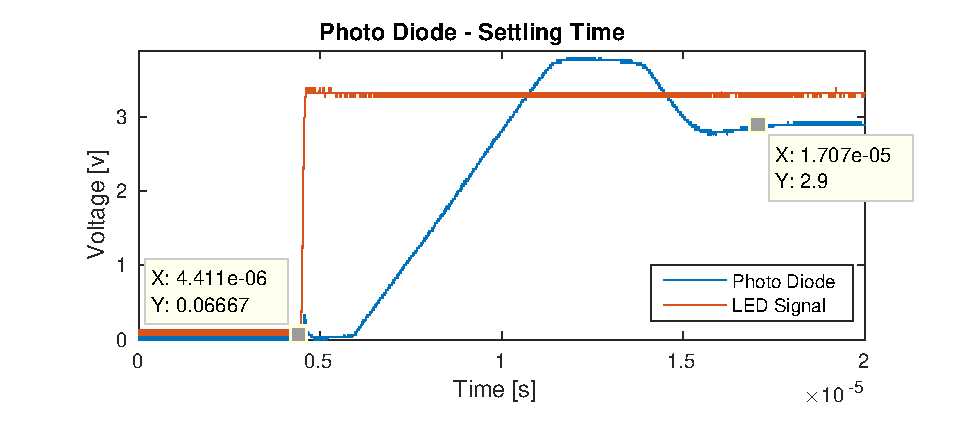
\includegraphics[width=\linewidth]{images/settle}
	\caption{Worst case settling time. When LED signal goes high, the photo diode is expected to have settled after $T_{\text{s}}=12.65\mu$s.}
	\label{fig:settletime}
\end{figure}

\subsection{LED Driver}
The LED driver is the VHDL component that contains the logic that determines which LED is on at any given time.
\begin{figure}[h!]
	\centering
	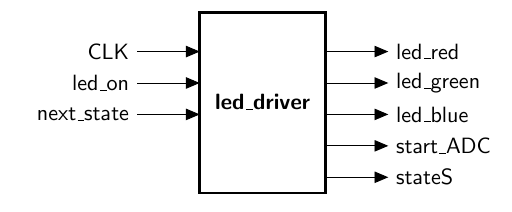
\includegraphics[scale=1]{images/LED_ent}
	\caption{heading}
	\label{fig:pinoutled}
\end{figure}
Only one LED is on at a time such that the reflection of each colour can be measured by the photodiode individually.
As mentioned in the previous section the LED has to be turned on for 13 $\mu$s such that output of the photodiode can settle such that the voltage is steady for the ADC conversion.
\subsection{Implementation of the LED driver}

The LED driver is implemented with 2 processes , \texttt{state\_changer} and \texttt{LED\_process}. 

\texttt{State\_changer} consists of a finite state machine, FSM, which has three states , \texttt{Red}, \texttt{Green}, \texttt{Blue} which each turn on their respective LED, and turn off the others.  The FSM start at \texttt{Red}.  At this state \texttt{led\_red} is set to high.\\

In \texttt{LED\_process}, \texttt{count} is incremented for each \texttt{rising\_edge} of \texttt{CLK}.  When \texttt{count} goes above 650, 13 $\mu$s have passed, and  \texttt{start\_ADC} is set high. 
\texttt{start\_ADC} is used to signal to the ADC component that a conversion is needed.
Once the conversion is completed, this will be signalled to the control module, see section \ref{sec:control}, which in turn will set \texttt{next\_state} high.
When \texttt{next\_state} goes high, \texttt{count} is reset, \texttt{start\_ADC} is set low  and the state machine progresses to the next state.
%% May have to remove LED_on.. Don't have to turn them off.. 
